% =============================================================================
% overview
% =============================================================================

To set the stage for what follows in this chapter, we first give a brief overview of some of the concepts in the \ER notation with the help of an example shown in \fig{eg1}. This example will be re-use throughout the description of the graphical symbols (glyphs) used by \SBGNERLone (with a few additions when the concepts are missing in the example) 

\begin{figure}[H]
  \centering
  \vspace*{-0.75em}
  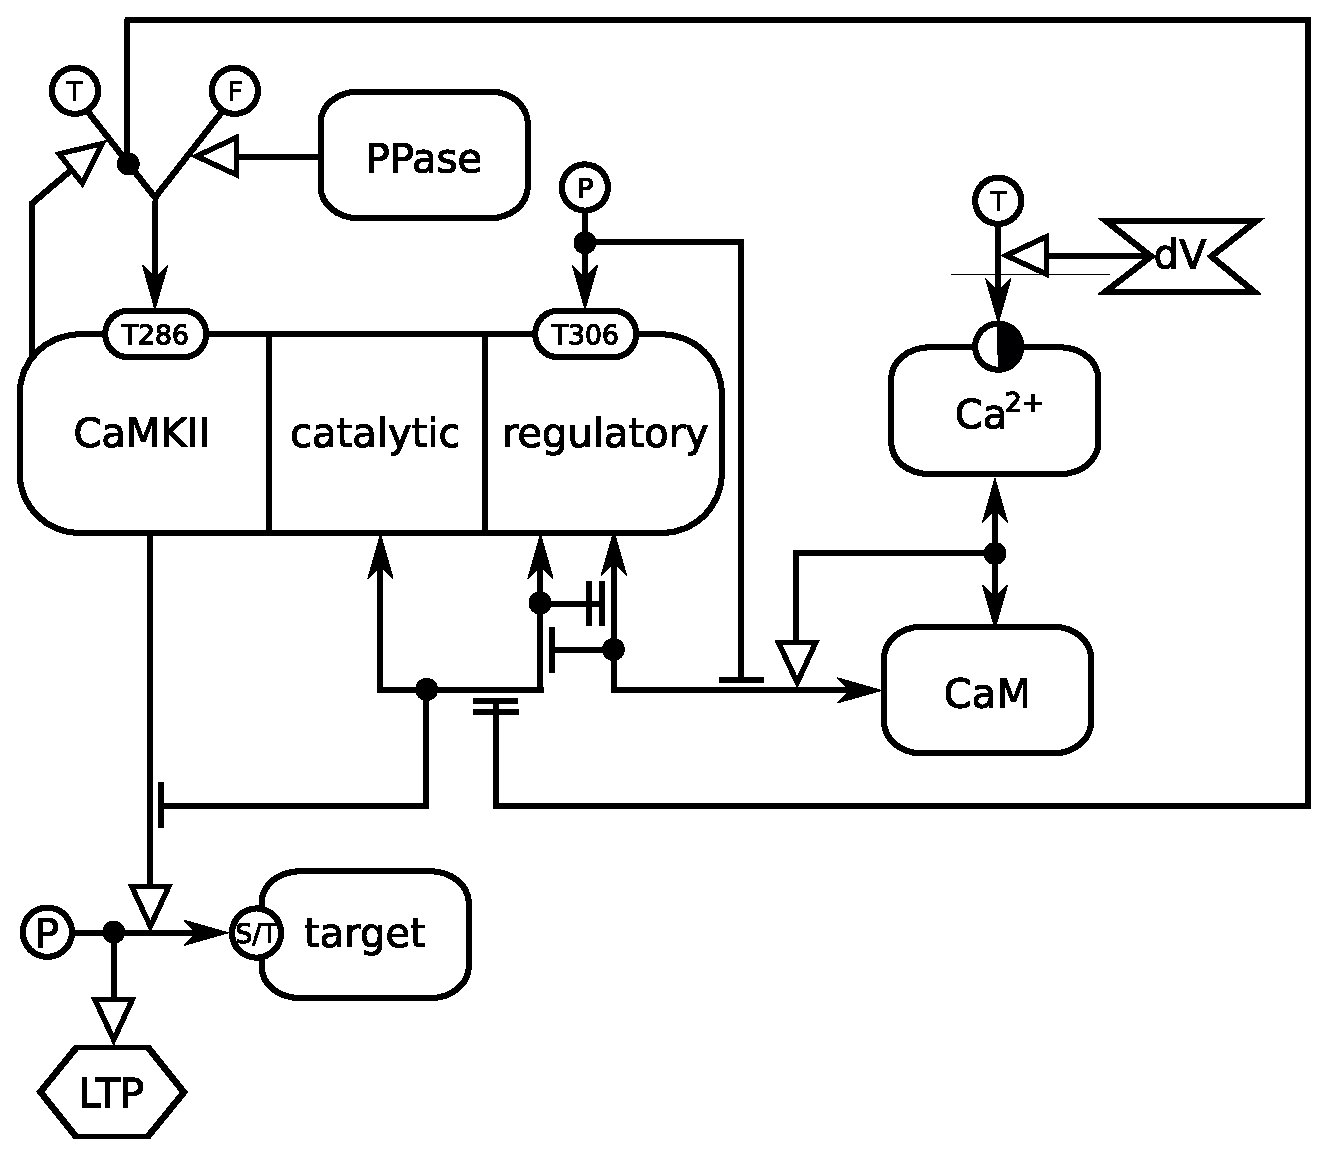
\includegraphics[scale=0.6]{examples/CaMKII-intro}
   \caption{This example of a \ER diagram depicts the effect of a depolarisation (dV) on the intracellular calcium, that binds to Calmodulin (CaM), that itself binds to the calcium/calmoduline kinase II (CaMKII). The binding of calmodulin inhibits the interaction between the catalytic and regulatory domains, thus relieving the inhibition on the kinase activity. The phosphorylation of the targets finally leads to the Long Term Potentiation (LTP) of the synapses. In addition, the diagram shows the effect of phosphorylation on threonine 286, that makes the enzyme constitutively active, and on threonine 306, that renders the kinase insensitive to calmodulin.}
  \label{fig:eg1}
\end{figure}
 
The essence of the \ER diagram is to depict the influences of entities upon the behaviour of others. The entities can exist or not, and the relationships can therefore be understood as logical consequences of this existence. Contrary to the Process Diagram notation, where the different processes affect each other, the relationships are independent. On can imagine that each of the relationships represent the conclusion of a scientific experience or article. The independence of relationships is the key to avoid the combinatorial explosion inherent to Process Diagrams.

% \tab{component-summary} summarizes the different SBGN abstractions described in this chapter.
% 
% \newcolumntype{P}[1]{>{\raggedright\hspace{0pt}\arraybackslash}p{#1}}
% 
% \begin{table}[bh]
%   \centering
%   \small
%   \begin{tabular}{@{}llP{2.4in}P{1.6in}@{}}
%     \toprule
%     \textbf{Component} & \textbf{Abbrev.} & \textbf{Role} & \textbf{Examples}\\
%     \midrule
%     Entity pool node
%     & EPN
%     & A population of entities that cannot be distinguished from each other
%     & Specific macromolecules or other chemical species \\[0.5em]
% 
%     Container node	
%     & CN
%     & An encapsulation of one or more other SBGN constructs
%     & Complexes, compartments \\[1.6em]
% 
%     Process node
%     & PN
%     & A process that transforms one or more EPNs into one or more other EPNs
%     & Transition, association, dissociation \\[0.5em]
% 
%     Connecting arc
%     & ---
%     & Links between EPNs or CNs to PNs or CNs to indicate influences
%     & Production, catalysis, inhibition \\[0.5em]
% 
%     Logical operators
%     & ---
%     & Combines one or several inputs into one output
%     & Boolean \emph{and}, \emph{or}, \emph{not} \\
%     \bottomrule
%   \end{tabular}
%   \caption{Summary of \PD components and their roles.}
%   \label{tab:component-summary}
% \end{table}

